\documentclass[letterpaper,12pt,twoside,]{pinp}

%% Some pieces required from the pandoc template
\providecommand{\tightlist}{%
  \setlength{\itemsep}{0pt}\setlength{\parskip}{0pt}}

% Use the lineno option to display guide line numbers if required.
% Note that the use of elements such as single-column equations
% may affect the guide line number alignment.

\usepackage[T1]{fontenc}
\usepackage[utf8]{inputenc}

% pinp change: the geometry package layout settings need to be set here, not in pinp.cls
\geometry{layoutsize={0.95588\paperwidth,0.98864\paperheight},%
  layouthoffset=0.02206\paperwidth, layoutvoffset=0.00568\paperheight}

\definecolor{pinpblue}{HTML}{185FAF}  % imagecolorpicker on blue for new R logo
\definecolor{pnasbluetext}{RGB}{101,0,0} %


\usepackage{wrapfig,subcaption,array,tabularx,multirow,caption}

\title{QBUS2820 Assignment 1}

\author[]{}


\setcounter{secnumdepth}{0}

% Please give the surname of the lead author for the running footer
\leadauthor{}

% Keywords are not mandatory, but authors are strongly encouraged to provide them. If provided, please include two to five keywords, separated by the pipe symbol, e.g:
 

\begin{abstract}

\end{abstract}

\dates{This version was compiled on \today} 

% initially we use doi so keep for backwards compatibility
% new name is doi_footer

\pinpfootercontents{QBUS2820 Assignment 1}

\begin{document}

% Optional adjustment to line up main text (after abstract) of first page with line numbers, when using both lineno and twocolumn options.
% You should only change this length when you've finalised the article contents.
\verticaladjustment{-2pt}

\maketitle
\thispagestyle{firststyle}
\ifthenelse{\boolean{shortarticle}}{\ifthenelse{\boolean{singlecolumn}}{\abscontentformatted}{\abscontent}}{}

% If your first paragraph (i.e. with the \dropcap) contains a list environment (quote, quotation, theorem, definition, enumerate, itemize...), the line after the list may have some extra indentation. If this is the case, add \parshape=0 to the end of the list environment.


\captionsetup[figure]{labelfont={it,bf,scriptsize},textfont={it,scriptsize},labelsep=colon}
\captionsetup[table]{labelfont={it,bf,scriptsize},textfont={it,scriptsize},labelsep=colon}
\captionsetup[FLOAT_TYPE]{labelformat=simple, labelsep=colon}

\hypertarget{task-a}{%
\section{Task A}\label{task-a}}

\hypertarget{introduction}{%
\section{Introduction}\label{introduction}}

Although the NBA is known for being a sport league across globe, it is a
vast economic entity as well. Undoubtedly, it has been a major impact in
the past decades, and it does not seem to be slowing down anytime soon.
Beside the League's branding, its commercial success is contributed by
the players at large as they make the trends on social media and attract
costumers to buy their products in a constance. However, the most
important attribute of a player is none other than his performance on
the court. Performance is what NBA players thrive for as it decides
their salary level. How much salary a player is worth can be a hard
estimation to the teams because the performance of athlete fluctuates.
Furthermore, the salary cap of the League as a whole, too, fluctuate
every year. Fortunately, the League records players' data in various
categories which include field goal attempted, field goal percentage,
offensive and defensive ratings, etc. With this data, machine learning
techniques can be applied to develop reliable models to predict salary
so that to help the NBA better performing their business manner such as
human resource management, financial management and marketing
strategies.

This project aims to develop predictive models of salary for NBA
basketball players. Three types of techniques including k-nearest
neignbour regression, linear regression and lasso regression are
involved. Predictive models are developed by changing corresponding
parameters and features, with 5-fold cross validation being applied to
assess root mean squared errors of these models. The optimal model is
then selected by the lowest validation error for each technique. With
the best predictive performance, a lasso regression model having the
lowest test set root mean squared error is found to be best-suited the
NBA data.

\hypertarget{data-processing-and-exploratory-data-analysis}{%
\section{Data processing and exploratory data
analysis}\label{data-processing-and-exploratory-data-analysis}}

Two datasets \texttt{NBA\_train} and \texttt{NBA\_test} are analysed in
this project. The data is collected by NBA, with the corresponding raw
data and metadata being publicly accessible on the NBA websites.

There are 2 categorical variables and 19 numeric variables regarding
players' personal information and game performance, with an additional
unique ID of each record in the datasets. The numeric variables includes
salary, age, number of games played , number of minutes played, personal
efficiency rate , true shooting percentage, offensive rebounds ,
defensive rebounds , turnover percentage , assists , steals, blocks ,
turnover percentage , usage percentage , offensive rating, defensive
rating and win shares while the categorical variables are the position
and the team a player in. The corresponding variable names can be found
the Table \ref{table:var}

The \texttt{NBA\_train} dataset is used for training and validating
predictive models in this project while the \texttt{NBA\_test} dataset
is used for testing selected models. Therefore the exploratory data
analysis is conducted based on the \texttt{NBA\_train} dataset.

\begin{wrapfigure}{r}{0.4\textwidth}
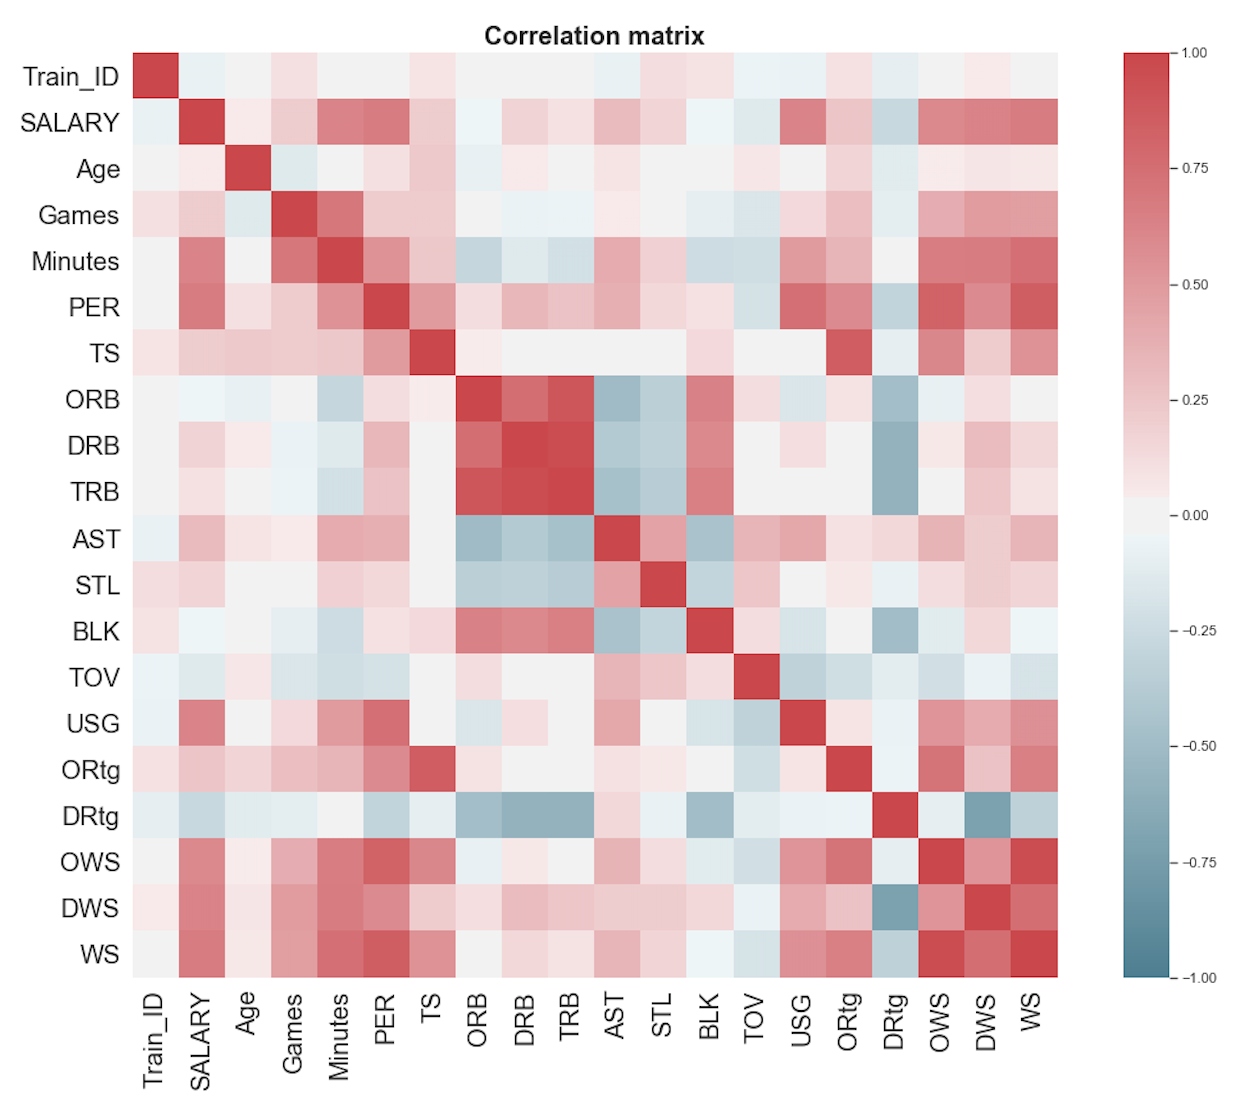
\includegraphics[width=1\linewidth]{correlation.png}
\centering
\caption{Correlations between numeric variables based on correlation coefficients.}
\label{fig:correlation}
\end{wrapfigure}

Figure \ref{fig:correlation} illustrate that win share, defensive win
share, offensive win share, number of minutes played and personal
efficiency rate show linear relationships with salary, with win share
having the strongest linear relationship with salary at a correlation
coefficient of 0.68. It also provides evidences of linearity between
offensive win share, defensive win share and win share. Although other
variables show mild linear relationship with salary, there can be other
linkage between salary and these variables. Thus variables showing no
linearity with salary can still be potentially informative and should be
left for further feature selection when developing predictive models.

Moreover, colinearity is observed between several variables. The number
of win shares which is linearly related to salary is also found to be
correlated with number of offensive win shares and number of defensive
win shares, while total rebound is linearly related to both offensive
rebound and defensive rebound.

The relationships between salary and the six relative variables as well
as the distribution of numeric variables are further visualized by a
scatter plot matrix. In Figure \ref{fig:scatter}, the linearity between
numeric variables and salary shown is in line with the correlation
matrix (Figure \ref{fig:correlation}). Moreover, salary, win share,
defensive win share and offensive win share are significantly
right-skewed while usage percentage and personal efficiency rate are
slightly right-skewed. In additions, the distributions demonstrates a
small variance of number of minutes played.

To analyse the categorical variables, box plots are generated to
visualize the distribution of salary. Figure \ref{fig:position}
describes how salary varies for players in different positions. Although
the median salaries are similar at \$4-6 millions for the five
positions, variances of salary are slightly different. Salaries for
players in the center and small forward position vary significantly
without any outliers whereas variances of salary for both power forward
and shooting guard are smaller with an outlier. Nevertheless, the
distributions of salary for players in different positions are similar.

Outlining in Figure \ref{fig:team}, salary varies across different
teams, which is reasonable in a business entity. There are many
basketball teams within the NBA, resulting in small sample sizes of
salary in each group. Some groups, such as Los Angeles Clippers, Phoenix
Surs and Denver Nuggets, have information of only one player being
recorded in this dataset. Furthermore, the team variable has no
intrinsic order, and the teams in any unseen data can contain new teams.
This makes the team variable less informative.

\begin{figure}[H]
\begin{subfigure}{0.5\textwidth}
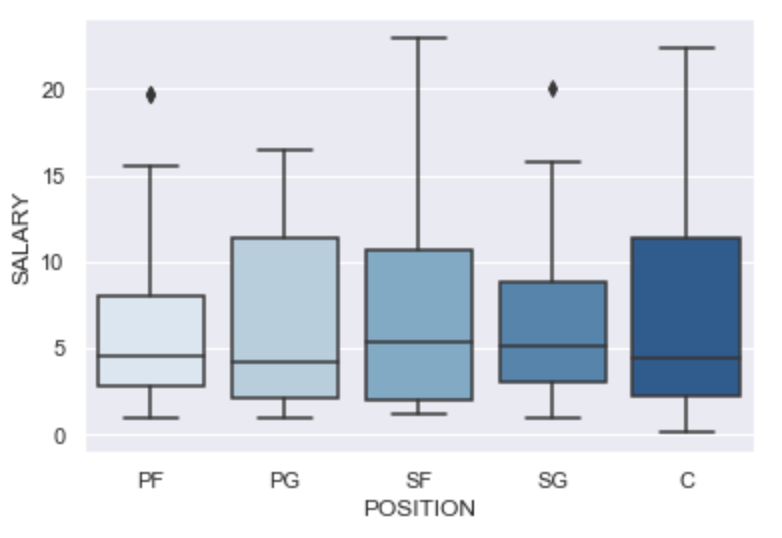
\includegraphics[width=0.9\linewidth, height=5cm]{position_box.png}
\centering
\caption{Salaries for players in different positions.}
\label{fig:position}
\end{subfigure}
\begin{subfigure}{0.5\textwidth}
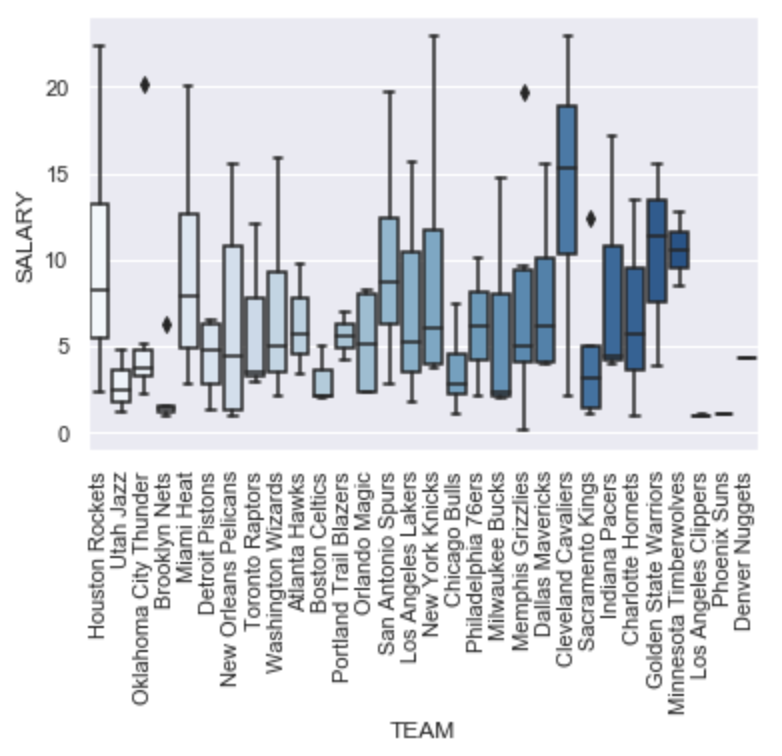
\includegraphics[width=0.9\linewidth, height=5cm]{team_box.png}
\centering
\caption{Salaries for players in different teams.}
\label{fig:team}
\end{subfigure}
\caption{Box plots of salaries for players in different teams and positions.}
\label{fig:boxes}
\end{figure}

\hypertarget{feature-engineering}{%
\section{Feature engineering}\label{feature-engineering}}

To discover any missing values involved in the datasets, bar charts of
missingness are generated to visualize missingness. As shown in Figure
\ref{fig:missingness}, both \texttt{NBA\_train} and \texttt{NBA\_test}
are complete without any missing values. Therefore no data removal or
data imputation is performed.

According to the results of exploratory data analysis, the record ID,
position a player in and team played are uninformative for predicting
salary. Therefore these three variables are discarded whereas the salary
is extracted from the \texttt{NBA\_train} and \texttt{NBA\_test}
datasets to be the response. There are 19 numeric features including
age, number of games played , number of minutes played, personal
efficiency rate , true shooting percentage, offensive rebounds ,
defensive rebounds , turnover percentage , assists , steals, blocks ,
turnover percentage , usage percentage , offensive rating, defensive
rating, win shares and team the player in, engaging in predictive model
development.

\hypertarget{methodology-of-k-nearest-neighbour-regression-models}{%
\section{Methodology of K-nearest neighbour regression
models}\label{methodology-of-k-nearest-neighbour-regression-models}}

The K-nearest neighbour regression models are trained by one of the 19
numeric features, with different values of K ranging from 1 to 50.
Totally 950 models are developed by changing the feature and the value
of k. 5-fold cross validation is applied to assess negative mean square
errors of models, followed by transferring negative mean square errors
to root mean square errors. The model with the smallest root mean square
error is selected as the optimal model.

\begin{wrapfigure}{r}{0.4\textwidth}
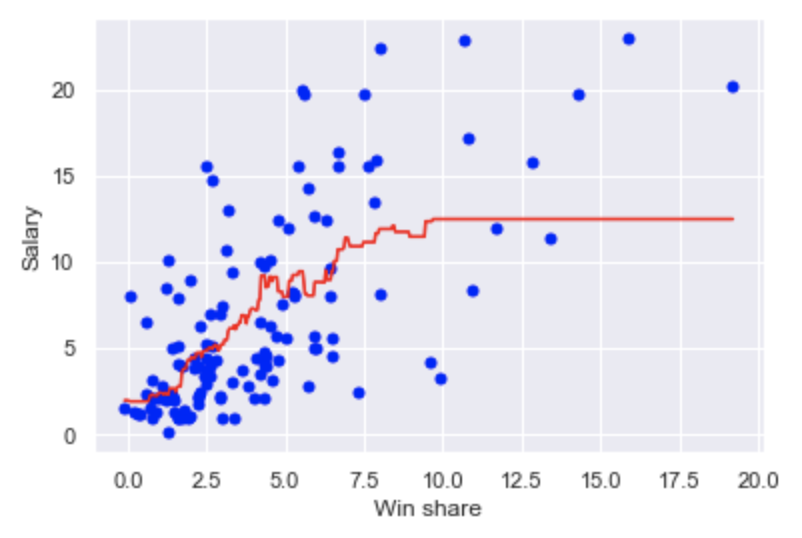
\includegraphics[width=1\linewidth]{knn_plot.png}
\centering
\caption{Visualizing the K-nearest neighbour model with K = 19 and number of win shares as the feature.}
\label{fig:knn}
\end{wrapfigure}

The model trained by the number of win shares and a k of 19, which has a
validation error of 4.2615 (\$ Millions), is chosen to be the optimal
K-nearest neighbour regression model. With this model, 19 neighbours are
considered to examine the value of salary with specific number of win
shares. Figure \ref{fig:knn} visualizes this k-nearest neighbour
regression model with observed data points of salary against number of
win shares. Generally, the salary is predicted to increase as number of
win shares increases, which is logical with the economic concern of the
NBA. The more games a player win, the more valuable he is in the
basketball team and thus the play deserves a higher salary. The model
predicts salary to remain stable when 10 win shares is reached, which is
not in line with observed data points. This may result from the small
number of data points with number of win shares greater than 10,
resulting in insufficient neigbours for k-nearest neighbour model
training.

\hypertarget{methodology-of-linear-regression-models}{%
\section{Methodology of linear regression
models}\label{methodology-of-linear-regression-models}}

The polynomial regression models are trained by one of the 19 numeric
features with a polynomial degree varying between 1 and 10. 190
polynomial regression models are developed by selecting different
feature and the polynomial degree of the model.

Multiple linear regression models are also developed with different
features. Recursive feature elimination (RFE) which is a feature
selection method is applied. It removes weakest features based on
corresponding coefficients of linear regression model until the required
number of features is reached. The dependencies and colinearity between
features are also captured and eliminated by this method. As discussed
in the exploratory data analysis, there is colinerity between number of
defensive win shares, offensive win shares and win shares, and between
total rebound, offensive rebound and defensive rebounds. In order to
avoid violating the assumption of multiple linear regression, the number
of offensive win share and defensive win shares, offensive rebound and
defensive rebound are removed from the feature pool for feature
selection, leading to 15 numeric variables remaining in the feature
pool. The number of features required for recursive feature elimination
varies from 1 to 15, as such simple linear regression models with one
feature are also estimated in this approach.

Negative mean square errors of these models are obtained by implementing
5-fold cross validation. Root mean square errors are then calculated to
determine the optimal models of polynomial linear regression and
multiple linear regression.

\begin{wrapfigure}{r}{0.4\textwidth}
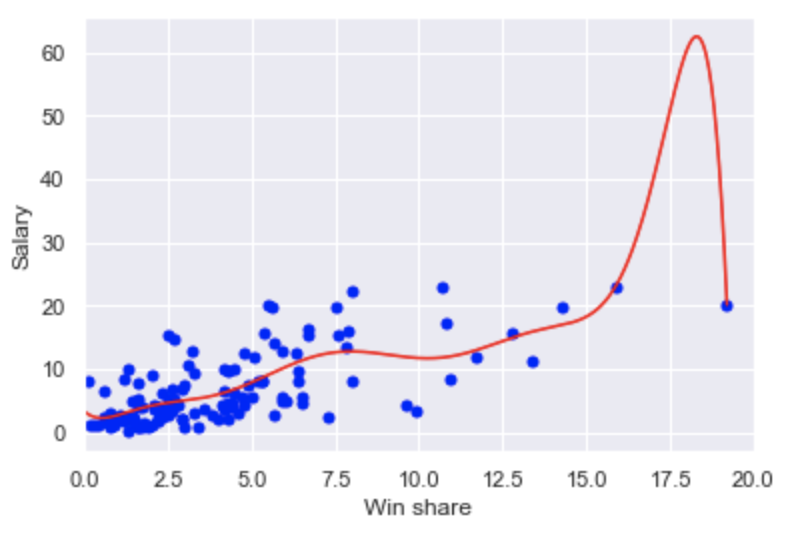
\includegraphics[width=1\linewidth]{poly_plot.png}
\centering
\caption{Visualizing the polynomial regression model and linear model with number of win share as feature. The polynomial regression model has a polynomial degree of 2.}
\label{fig:poly}
\end{wrapfigure}

The optimal polynomial regression model contains number of win shares as
the feature and a polynomial degree of 2. The predictive function of the
model is: \(Salary=1.4213+1.4339~WS-0.0219~WS^2\), where \(WS\) is the
number of win shares. As shown in Figure \ref{fig:poly}, The polynomial
regression better fits the observed data compared to the linear
regression model as it captures more variance of salary with regard to
different number of win shares.

The optimal multiple regression model involves 14 numeric features,
having the root mean square error of 3.792 (\$ Millions). The predictive
function is
\(Salary = 10.53-0.1~Age-0.16~Games+0.0037~Minutes-0.25~PER-0.098~TS+0.2~TRB-0.062~AST+0.58~STL-0.21~BLK+0.12~TOV+0.51~USG+0.11~ORtg-0.19~DRtg+0.49~WS\),
where salary rises with incrase in number of minutes played, total
rebounds, number of steals, turnover percentage, usage percentage,
offensive rating, win shares, and decrease in age, number of games
played, personal efficiency rating, true shooting percentage, assists,
blocks, defensive rating.

With a smaller root mean square error of training model, the optimal
multiple linear regression model including 14 features are finally
selected as the optimal linear regression model.

\hypertarget{methodology-of-lasso-regression-models}{%
\section{Methodology of lasso regression
models}\label{methodology-of-lasso-regression-models}}

Least absolute shrinkage and selection operator (Lasso), as an extension
of liner regression analysis, conducts both feature selection and
regularization. This helps to enhance the predictive performance and
interpretability of the model developed.

The objective of a lasso regression model is to minimize
\(\sum^n_{i=1}(y_i-\sum_jx_{ij}\beta_j)^2+\alpha\sum^p_{j=1}|\beta_j|\),
where \(\alpha\) is a tuning parameter which represents how strong the
L1 regularization penalize coefficients of the lasso regression model.
Changing the value of \(\alpha\) influences the number of features
eliminated. When \(\alpha=0\), coefficients of features are not
Palisades such that no feature is removed. As the value of \(\alpha\)
increases, L1 penalty gets stronger and therefore more features are
eliminated, vice versa. Furthermore, the value of \(\alpha\) also
affects the bias-variance trade-off. An increase of \(\alpha\) leads to
increase in bias while a decrease of \(\alpha\) results in increase in
variance.

Lasso regression model automates feature selection whereas multiple
linear regression model require additional feature selection approach to
deal with multicollinearity. Moreover, L1 regularization which penalizes
the coefficients of linear regression model is performed with lasso
regression. In the source data of this project, outliers and
multicollinearity exist in several pairs of features. In this case,
lasso regression with automated feature selection and regularization
could be better-suited for the data compared to regular linear
regression.

Lasso regression is a supervised learning technique while K-nearest
neighbour regression is an unsupervised learning technique, which means
a linear function is pre-defined for lasso regression when K-nearest
neighbour regression observes pattern in the data without fix function.
As such, lasso regression is more interpretable but less flexible than
k-nearest neighbour regression. In this project, one of the goals is to
discover dominant factors of salary for NBA players. To achieve this
goal, a lasso regression model which can clearly define weights of
features is more powerful compared to a KNN regression model.

19 numeric features are fed into lasso regression models with 7 values
of alpha: 0.0001, 0.001, 0.01, 0.1, 0.5, 5 and 10. 5-fold cross
validation is then applied to assess predictive performance of models.
The optimal lasso model is selected based on negative mean squared
error, the smaller the negative mean squared error, the better the lasso
model performs.

The optimal value of \(\alpha\) is 0.5 for this data. With this value of
\(\alpha\), 10 features are selected with the predictive function:
\(Salary = 25.18-0.0044~Age-0.18~Games+0.0056~Minutes+0.1~PER+0.036~DRB-0.054~AST+0.098~TOV+0.27~USG-0.23~RDtg+0.17~WS\).
This indicates that salary increases with increases in number of minutes
played, personal efficiency rate, defensive rebounds, turn over
percentage, usage percentage and number of win shares while decreases in
age, number of games played, assists and defensive rating result in an
increase in salary. The validation root mean squared of the model is
-12.8575 (\$ Millions), which is the best performance among 7 lasso
regression models developed.

\hypertarget{test-set-performance}{%
\section{Test set performance}\label{test-set-performance}}

Root mean squared error is used to assess the predictive performance of
three models selected.

The selected k-nearest neighbour regression model has a test set root
mean squared error of 4.2288, representing a standard deviation of
unexplained variance of salary at 4.2288 millions dollars.

The selected multiple linear regression model has a test set error at
4.0532, indicating that the standard deviation of the unexplained
variance of salary by the multiple linear regression is 4.0532 millions
dollars.

The test set error of the optimal lasso regression model is 3.9570,
demonstrating a standard deviation of uncaptured variance of salary by
the lasso regression at 3.9570 millions dollars.

With the rule of thumb of 4.1 millions dollars, the predictive
performances of the multiple linear regression model with 14 features
and the lasso regression model with \(\alpha=0.5\) are satisfactory.

\begin{wraptable}{r}{8cm}
\begin{tabular}{ |c|c|c|c| } 
\hline
\textbf{Model} & \textbf{Validation error} & \textbf{Test set error} \\
\hline
\textbf{KNN regression} & 4.2615 & 4.2288 \\ 
\textbf{Multiple linear regression} & 3.7920 & 4.0532 \\
\textbf{Lasso regression} & 3.5857 & 3.9570 \\
\hline
\end{tabular}
\centering
\caption{Summary of training and testing performance of three predictive models. Both validation error and testing errors are estimated by root mean squared error.}
\label{table:errors}
\end{wraptable}

As shown in Table \ref{table:errors}, a predictive model with a lower
validation error tends to have a lower testing error. The lasso
regression model with \(\alpha=0.5\) has the lowest testing error, at
3.957 millions dollars. Therefore generally the lasso regression model
is the best-suited the data with greatest predictive performance.

\hypertarget{analysis-and-conclusions}{%
\section{Analysis and conclusions}\label{analysis-and-conclusions}}

In conclusion, predictive performance can vary significantly with
different features and parameters of machine learning techniques. The
optimal multiple linear regression model contains 14 features while the
optimal lasso regression model selects 10 features and a \(\alpha\)
value of 0.5. These two models satisfies the predictive performance rule
of thumb which requires root mean squared errors less than 4.1 millions
dollars.

Although the 19-nearest neighbour regression model with win shares as
feature is the optimal knn model, it is not satisfactory with a
relatively high test set error compared to other techniques. With
regards to previous discussion, a limitation of the optimal k-nearest
neighbour model is that it does not accurately predict salary for a
large number of win shares because of the outliers. This can also be the
main reason of the undesired predictive performance. A potential
solution to this issue is to choose a smaller values of k so that the
salary is estimated based on fewer neibours. However, this could worsen
predictive performance of the whole model as root mean squared error
increases. More attention should be paid on this trade-off in further
study. Another solution could be scaling the salary with logorithm to
deal with outliers. Moreover, a problem of whether and how the feature
selection should be perform for k-nearest neighbour is yet to be
discussed.

\hypertarget{appendix}{%
\section{Appendix}\label{appendix}}

\begin{table}[ht]
\centering
\begin{tabular}{ |c|c|c|} 
\hline
\textbf{Variables} & \textbf{Description} & \textbf{Data type}\\
\hline
ID & Unique identification number of the record & Numeric\\ 
SALARY & Salary for the NBA player & Numeric \\
POSITION & Position played & Categorical \\
TEAM & Team the player in & Categorical \\
Age & Age of the player & Numeric \\
Games & Number of games played & Numeric \\
Minutes & Number of minutes played & Numeric  \\
PER & Personal efficiency rate & Numeric  \\ 
TS & True shooting percentage & Numeric  \\
ORB & Offensive rebounds & Numeric  \\
DRB & Defensive rebounds & Numeric  \\
TRB & Total rebounds & Numeric  \\
AST & Number of assists & Numeric  \\
STL & Number of steals & Numeric  \\
BLK & Number of blocks & Numeric  \\
TOV & Turnover percentage & Numeric  \\
USG & Usage percentage & Numeric  \\
ORtg & Offensive rating & Numeric  \\
DRtg & Defensive rating & Numeric  \\
OWS & Offensive win shares & Numeric  \\
DWS & Defensive win shares  & Numeric \\
WS & Win shares & Numeric  \\
\hline
\end{tabular}
\centering
\caption{Table of variables.}
\label{table:var}
\end{table}

\begin{figure}
\begin{subfigure}{0.55\textwidth}
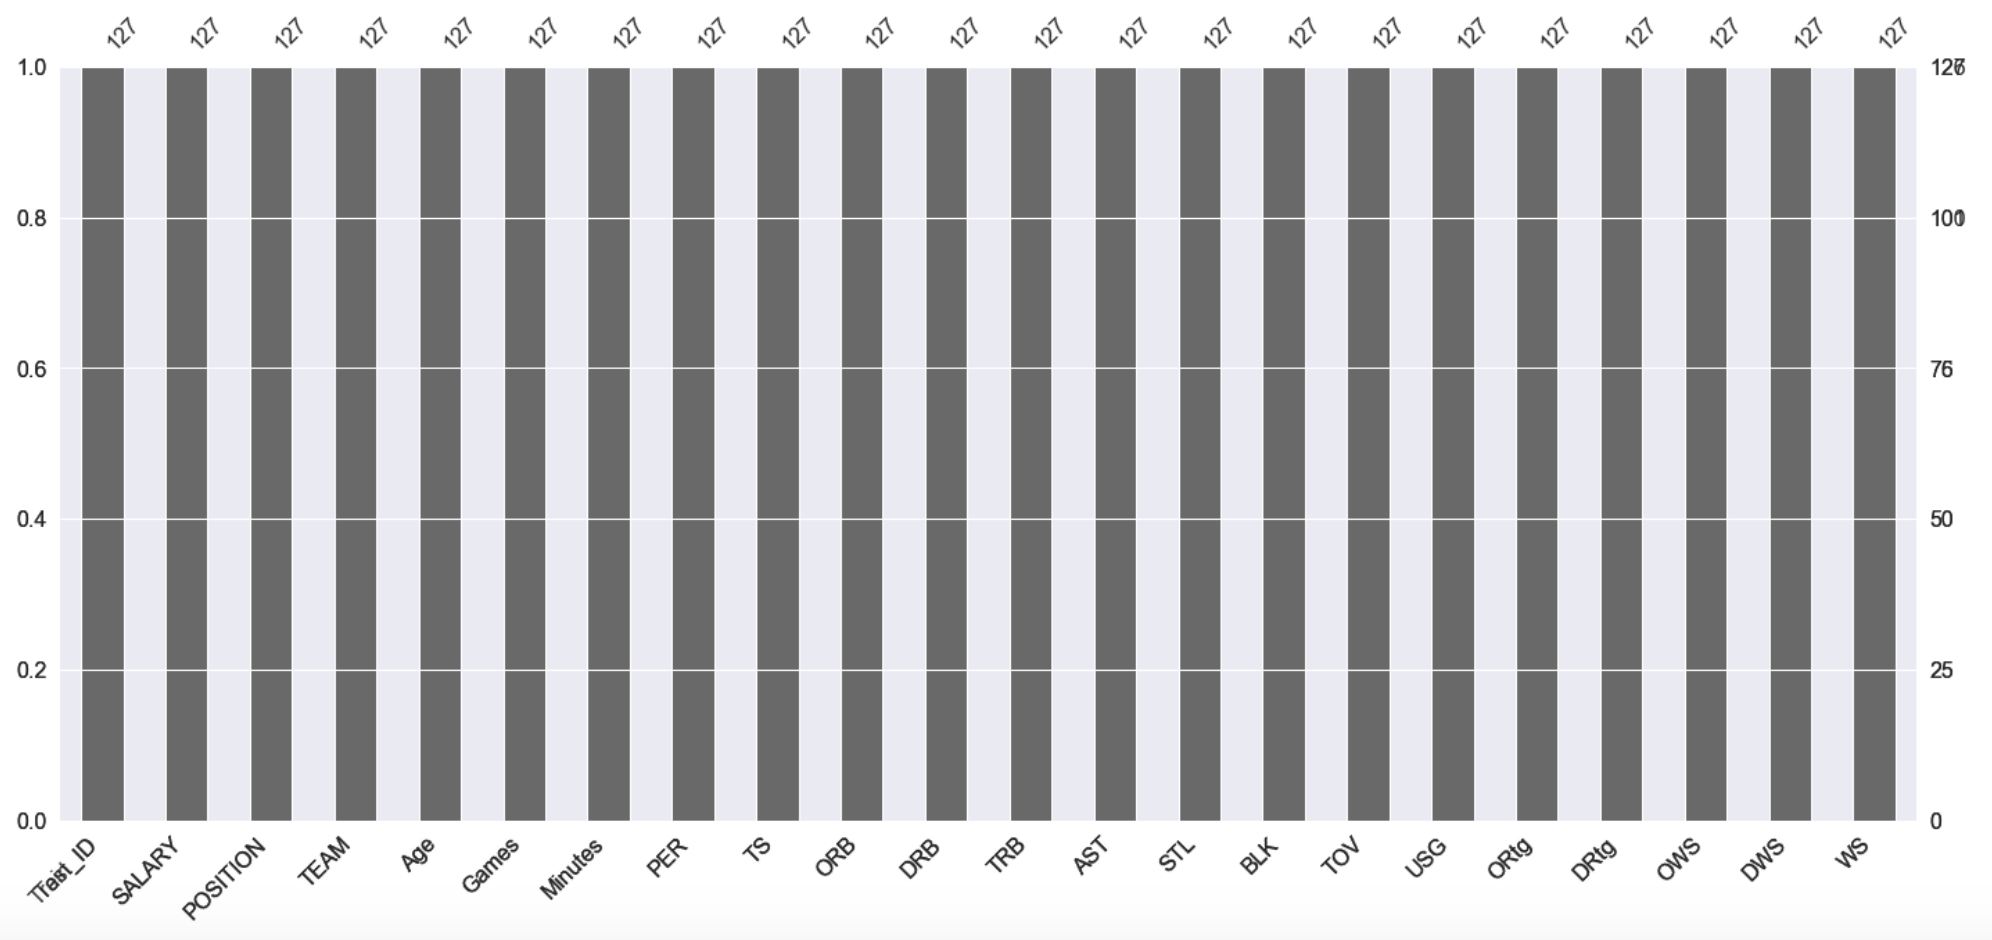
\includegraphics[width=0.9\linewidth, height=5cm]{nbaTrain_miss.png} 
\caption{Missingness bar chart of the `NBA train` dataset.}
\label{fig:trainMiss}
\end{subfigure}
\begin{subfigure}{0.55\textwidth}
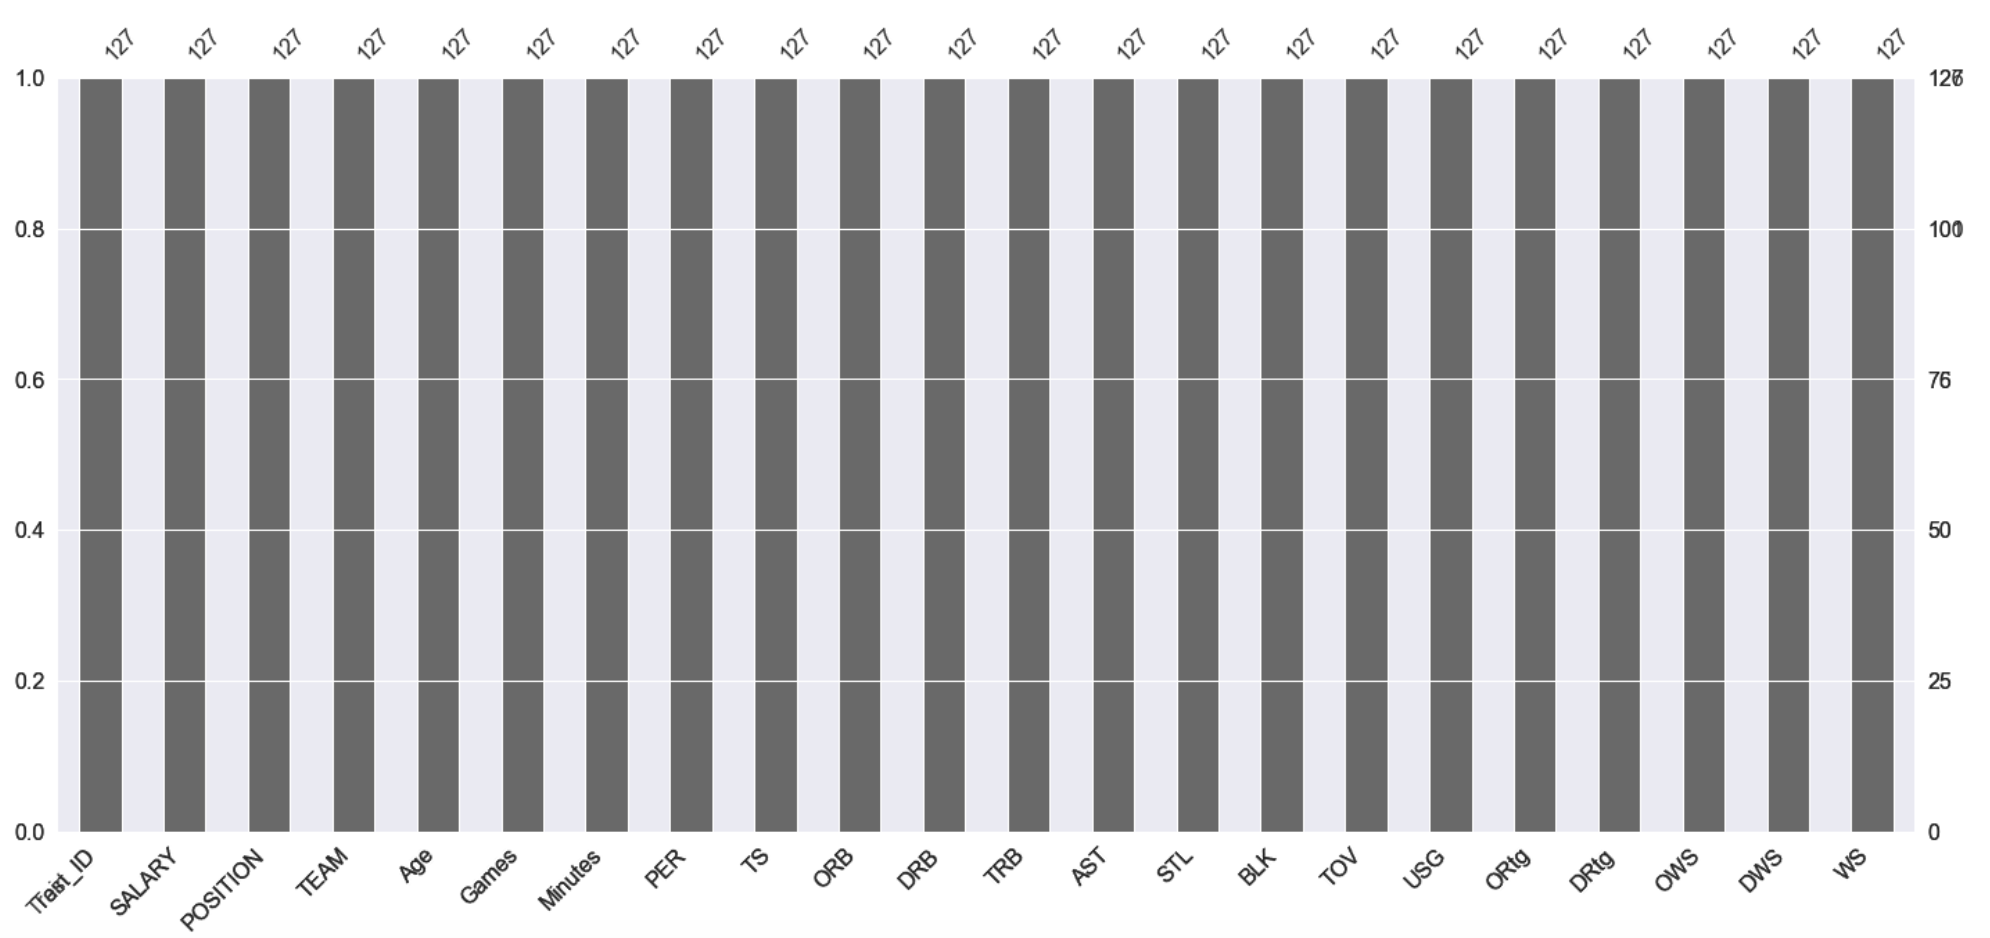
\includegraphics[width=0.9\linewidth, height=5cm]{nbaTest_miss.png}
\caption{Missingness bar chart of the `NBA test` dataset.}
\label{fig:testMiss}
\end{subfigure}
\caption{Visualizing the missingness of two datasets used.}
\label{fig:missingness}
\end{figure}

\begin{figure}
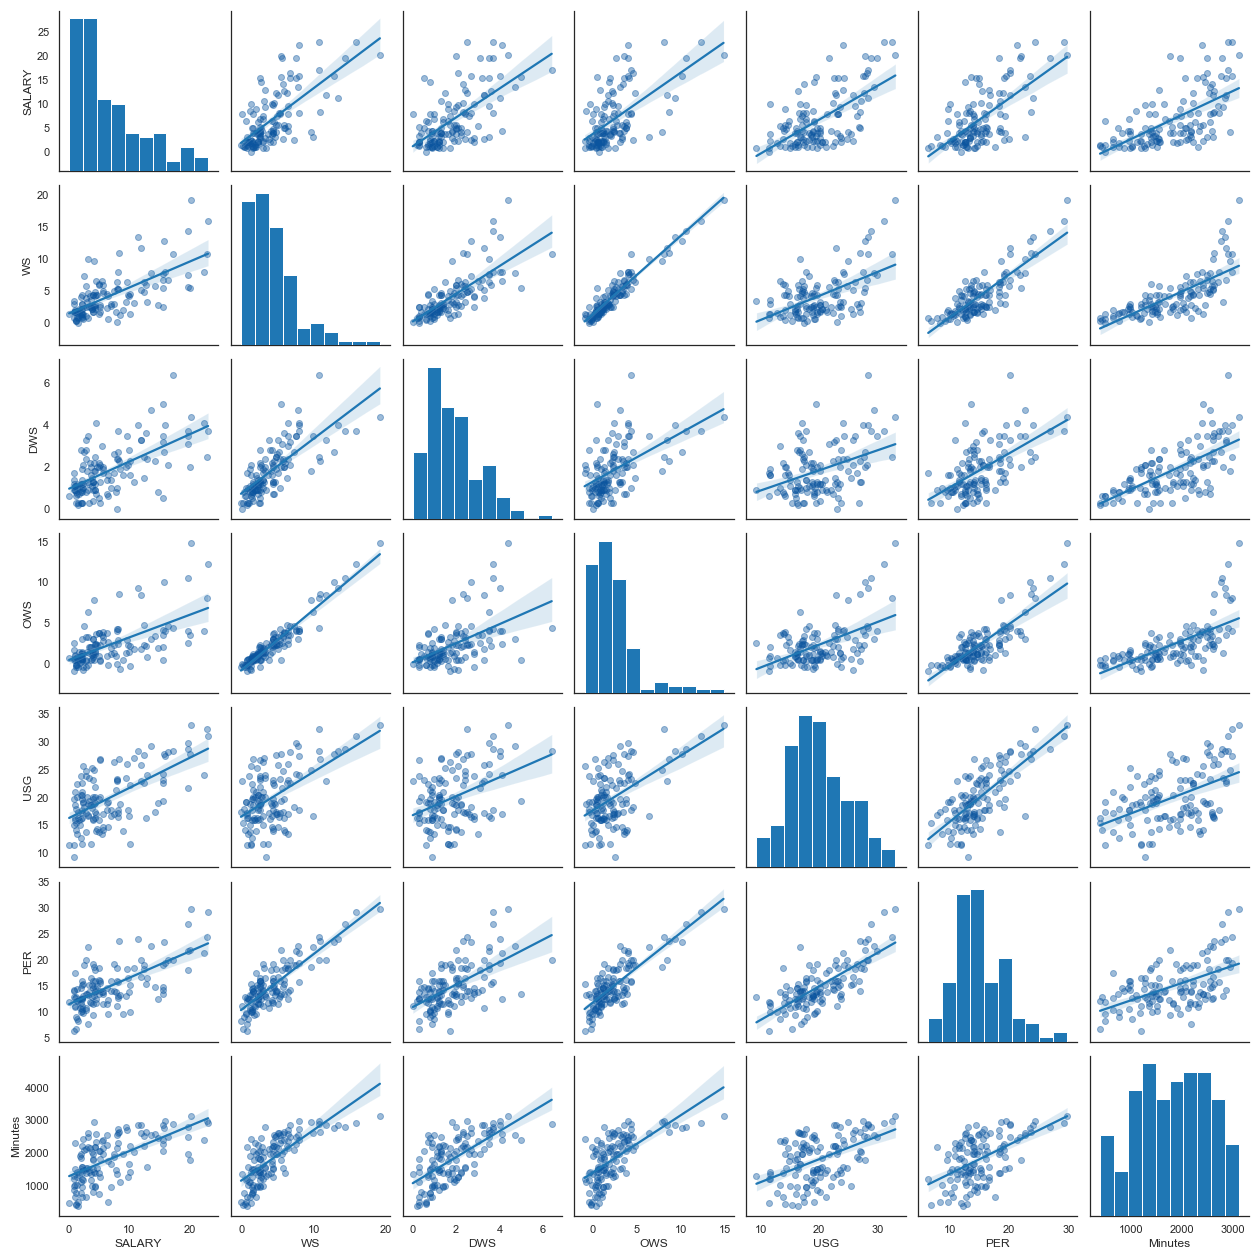
\includegraphics[width=0.85\textwidth]{scatter.png}
\centering
\caption{Distribution of numeric variables.}
\label{fig:scatter}
\end{figure}

\hypertarget{references}{%
\section{References}\label{references}}

\begin{itemize}
\item
  Pedregosa, F., et al. (2011). ``Scikit-Learn: Machine Learning in
  Python.'' Journal of Machine Learning Research, vol.~12,
  pp.~2825--2830.
\item
  Stephanie (2015). Lasso Regression: Simple Definition. {[}online{]}
  Statistics How To. Available at:
  \url{https://www.statisticshowto.com/lasso-regression/\#}:\textasciitilde{}:text=Lasso\%20regression\%20is\%20a\%20type.
\item
  Bilogur, (2018). Missingno: a missing data visualization suite.
  Journal of Open Source Software, 3(22), 547,
  \url{https://doi.org/10.21105/joss.00547}.
\item
  NBA Stats. (2018). NBA Stats. {[}online{]} Available at:
  \url{https://stats.nba.com/}.
\item
  Rençberoğlu, E. (2019). Fundamental Techniques of Feature Engineering
  for Machine Learning. {[}online{]} Medium. Available at:
  \url{https://towardsdatascience.com/}.
\item
  Wikipedia Contributors (2019). Lasso (statistics). {[}online{]}
  Wikipedia. Available at:
  \url{https://en.wikipedia.org/wiki/Lasso_(statistics)}.
\item
  Richards, J. (2020). Why We Use an 80/20 Split for Training and Test
  Data Plus an Alternative Method. {[}online{]} Medium. Available at:
  \url{https://towardsdatascience.com/}.
\item
  Basketball-Reference.com. NBA Win Shares. {[}online{]} Available at:
  \url{https://www.basketball-reference.com/about/ws.html}.
\end{itemize}

\clearpage

\hypertarget{task-b}{%
\section{Task B}\label{task-b}}

\hypertarget{exploratory-data-analysis}{%
\section{Exploratory data analysis}\label{exploratory-data-analysis}}

There are 14 numeric variables in the \texttt{Boston\ housing} dataset.
As shown in Figure \ref{fig:missHouse}, the dataset is 100\% complete
without missing values. \textbf{Outliers}

\begin{wrapfigure}{r}{0.4\textwidth}
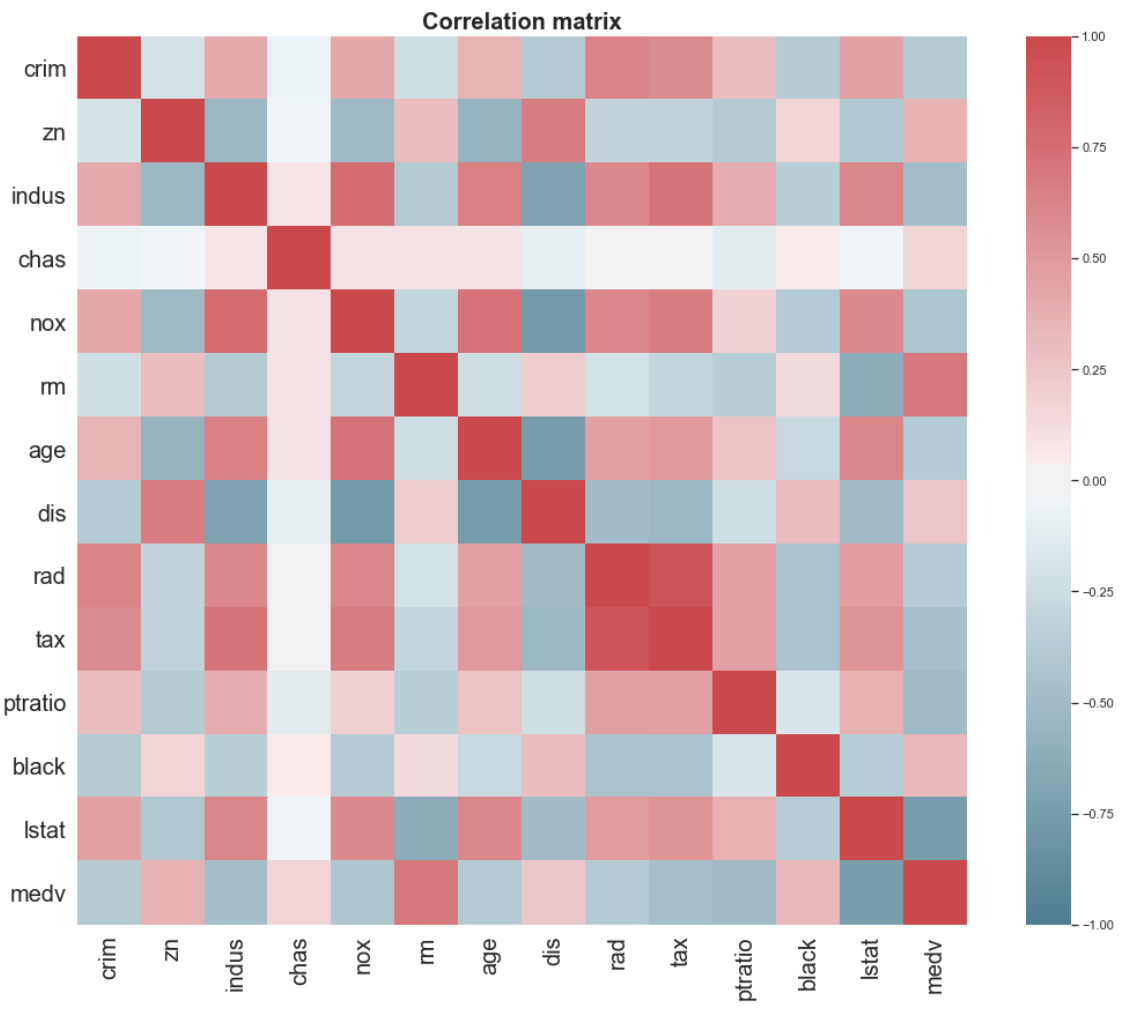
\includegraphics[width=1\linewidth]{house_corr.png}
\centering
\caption{Correlations between numeric variables in `Boston Housing` dataset.}
\label{fig:corrHouse}
\end{wrapfigure}

From Figure \ref{fig:corrHouse} and Table \ref{table:corrTab},
``lstat'', ``rm'' and ``ptrtio'' have relatively strong linear
relationship with ``medv''.

\begin{wrapfigure}{r}{0.4\textwidth}
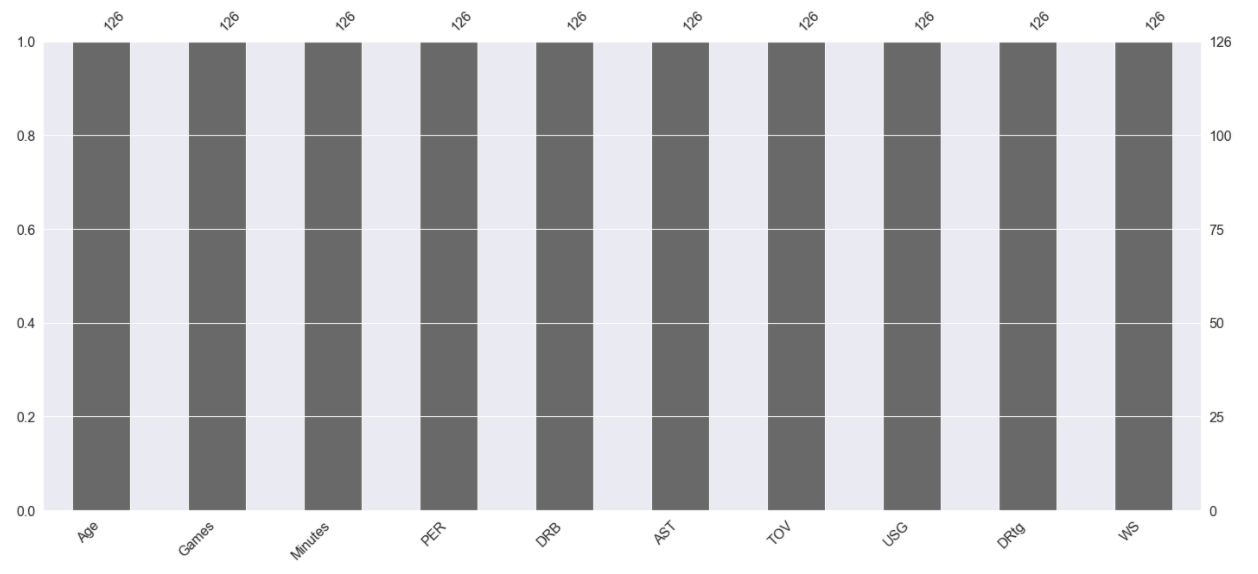
\includegraphics[width=1\linewidth]{miss_house.png}
\centering
\caption{Bar chart of missingness for `Boston housing` dataset.}
\label{fig:missHouse}
\end{wrapfigure}

\textbf{feature selection criteria}

\textbf{explain optimal learning rate}

\textbf{explain and justify approach}

\hypertarget{gradient-ascent-algorithm}{%
\section{Gradient ascent algorithm}\label{gradient-ascent-algorithm}}

\hypertarget{appendix-1}{%
\section{Appendix}\label{appendix-1}}

\begin{table}[ht]
\centering
\begin{tabular}{ |c|c|c|} 
\hline
\textbf{Variables} & \textbf{Correlation with "medv"} & \textbf{Absolute coefficient}\\
\hline
chas & 0.1753 & 0.1753 \\
dis & 0.2499 & 0.2499 \\
black & 0.3335 & 0.3335 \\
zn & 0.3604 & 0.3604 \\
age & -0.3770 & 0.3770 \\
rad & -0.3816 & 0.3816 \\
crim & -0.3883 & 0.3883 \\
nox & -0.4273 & 0.4273 \\
tax &-0.4685 & 0.4685 \\
indus & -0.4837 & 0.4837 \\
ptratio & -0.5078 & 0.5078 \\
rm & 0.6954 & 0.6954 \\
lstat & -0.7377 & 0.7377 \\
\hline
\end{tabular}
\centering
\caption{Correlation coefficients between "medv" and other variable in `Boston housing` dataset.}
\label{table:corrTab}
\end{table}

%\showmatmethods


\bibliography{pinp}
\bibliographystyle{jss}



\end{document}

